%% LyX 2.4.4 created this file.  For more info, see https://www.lyx.org/.
%% Do not edit unless you really know what you are doing.
\documentclass[english]{article}
\usepackage[T1]{fontenc}
\usepackage[latin9]{inputenc}
\usepackage{enumitem}
\usepackage{amsmath}
\usepackage{amsthm}
\usepackage{geometry}
\geometry{verbose,tmargin=1in,bmargin=1in,lmargin=1in,rmargin=1in}

\makeatletter
%%%%%%%%%%%%%%%%%%%%%%%%%%%%%% Textclass specific LaTeX commands.
\numberwithin{equation}{section}
\numberwithin{figure}{section}
\newlength{\lyxlabelwidth}      % auxiliary length 

%%%%%%%%%%%%%%%%%%%%%%%%%%%%%% User specified LaTeX commands.
\usepackage{fancyhdr}
\usepackage{lastpage}
\pagestyle{fancy}
\usepackage{enumitem}
\usepackage{ifthen}
\everymath=\expandafter{\the\everymath\displaystyle}
%\DeclareMathSizes{10}{10}{10}{10}
\usepackage{multicol}

\usepackage{tikz}
\usepackage{tikz-3dplot}
\usetikzlibrary{calc,arrows}

\usetikzlibrary{patterns}
\usetikzlibrary{plotmarks}
\usepackage{pgfplots}
\pgfplotsset{compat=newest}
\usepgfplotslibrary{polar}

\usepackage{calc}
\usepackage[nomessages]{fp}

\usepackage{datetime}
% Added by lyx2lyx
\setlength{\parskip}{\smallskipamount}
\setlength{\parindent}{0pt}

\makeatother

\usepackage{babel}
\begin{document}
\renewcommand{\author}{Dr.\,James Ashe}

\newcommand{\classNum}{331}

\newcommand{\classSec}{A}

\newcommand{\nameType}{Name:}

\newcommand{\examType}{Final Exam}

\renewcommand{\date}{\formatdate{3}{12}{2013}} %%\today

%%First page's header%%%%%%%%%%%%%%%%%%%%%%
\fancypagestyle{firststyle} %%header settings for first pagr
{
	\fancyhead[L]{MTH \classNum{}(\classSec{}) \author{}\\
	\textbf{\examType{}} \date{}}
	\fancyhead[C]{\textbf{\nameType}}
	\setlength{\headsep}{14pt}
}
%%%%%%%%%%%%%%%%%%%%%%%%%%%%%%%%%%%%%%%%%%

%%Next page's header%%%%%%%%%%%%%%%%%%%%%%%
\setlist{nolistsep}
\lhead{MTH \classNum{}(\classSec{})} 
\chead{\textbf{\nameType}} 
\cfoot{\thepage{}~of~\pageref{LastPage}} 
\setlength{\headsep}{5pt} 
%%%%%%%%%%%%%%%%%%%%%%%%%%%%%%%%%%%%%%%%%%%

%%Various settings; see the preamble for other settings%%%%%
%%\setenumerate[0]{leftmargin=12pt,itemindent=0pt,labelwidth=0pt}
\renewcommand{\labelenumi}{\textbf{\arabic{enumi}.}}
\renewcommand{\labelenumii}{\textbf{\alph{enumii}.}}
\thispagestyle{firststyle}

\newcommand{\xspace}{\vspace{1cm}}
\newcounter{probs}
%%%%%%%%%%%%%%%%%%%%%%%%%%%%%%%%%%%%%%%%%%

\textbf{Show your work. All problems are worth 4 point unless stated
otherwise.}
\begin{enumerate}[resume]
\item Write the expression, $x+x^{2}+x^{3}+x^{4}+\cdots+x^{20}$ in sigma
notation.\vfill\addtocounter{probs}{1}
\item Write out the following sum ${\displaystyle \sum_{n=0}^{3}n^{2}}$.\vfill\addtocounter{probs}{1}
\end{enumerate}
\emph{Evaluate the geometric series or state that it diverges. }
\begin{enumerate}[resume]
\item ${\displaystyle \sum_{k=0}^{\infty}\frac{1}{4^{k}}}$\vfill\addtocounter{probs}{1}
\item ${\displaystyle \sum_{m=0}^{\infty}\frac{(-3)^{2n}}{5^{n}}}$\vfill\addtocounter{probs}{1}
\end{enumerate}
\emph{Using the Squeeze Theorem, find the limit of the following sequence
or determine that the limit does not exist.}
\begin{enumerate}[resume]
\item ${\displaystyle \lim_{n\rightarrow\infty}\left\{ \frac{(-1)^{n}}{n}\right\} }$\vfill\addtocounter{probs}{1}
\end{enumerate}
\emph{Use the Divergence Test to determine whether the following series
diverge, or state that the test is inconclusive.}
\begin{enumerate}[resume]
\item ${\displaystyle \sum_{k=0}^{\infty}\frac{1}{k+1}}$\vfill\addtocounter{probs}{1}
\end{enumerate}
\newpage
\begin{enumerate}[resume]
\item Let $f(x)=3e^{x}$. (Each part is worth 4 points.)

\begin{enumerate}[resume]
\item Find the Taylor polynomial of order $n=2$ for $f(x)$ centered at
$0$.\vfill\addtocounter{probs}{1}
\item Use the Taylor polynomial from above to approximate $3e^{0.1}$, and
compute the absolute error in the approximation assuming the exact
value is given by a calculator.\vfill\addtocounter{probs}{1}
\end{enumerate}
\end{enumerate}
\emph{Give a set of parametric equations that describes the curve.}
\begin{enumerate}[resume]
\item Give two different sets of parametric equations that generate a circle
centered at $(0,0)$ with radius $5$.

\begin{enumerate}[resume]
\item {[}2 pts{]} Set one:\vspace{1cm}\addtocounter{probs}{1}
\item {[}2 pts{]} Set two:\vspace{1cm}\addtocounter{probs}{1}
\end{enumerate}
\end{enumerate}
\emph{Locate the following polar coordinates on a graph. }
\begin{enumerate}[resume]
\item A:$\left(1.5,\frac{\pi}{6}\right)$, B:$\left(1.5,\frac{\pi}{6}+\frac{\pi}{2}\right)$,
C:$\left(1.5,-\frac{\pi}{6}\right)$, D:$\left(-1.5,-\frac{\pi}{6}\right)$

\begin{enumerate}[resume]
\item []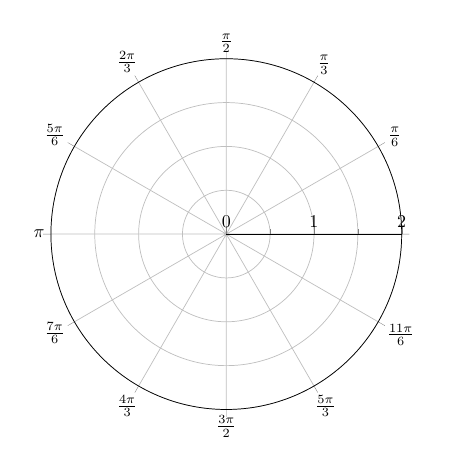
\begin{tikzpicture} [scale=.65] 
	\begin{polaraxis}[
			xmin=0,xmax=360,
			ymin=0,ymax=2,
			ytick={0,1,...,20}, 
			%minor x tick num={4},
			minor y tick num={1},
			grid=both,
			%yticklabels={,,,1,,,2,,}, 
			xticklabels={,,$\frac{\pi}{6}$,$\frac{\pi}{3}$,$\frac{\pi}{2}$,$\frac{2\pi}{3}$,$\frac{5\pi}{6}$,$\pi$,$\frac{7\pi}{6}$,$\frac{4\pi}{3}$,$\frac{3\pi}{2}$,$\frac{5\pi}{3}$,$\frac{11\pi}{6}$,}
		]
		%\addplot+[black, very thick, mark=none, domain=0:720, samples=600 ] {2-5*cos(x)};
		%\addplot+[gray, very thin, mark=none, domain=0:720, samples=600 ] {1.5};
		%\addplot+[black, mark = *, nodes near coords=mylabel,every node near coord/.style={anchor=180}] coordinates ( 30: 1.5);
		%\draw (30:1.5) circle[radius=2pt];
		%\addplot[color=blue,solid,mark=*,very thick] coordinates {(30,1.5)} node[below] {\large{A, D}};
		%\addplot[color=blue,solid,mark=*] coordinates {(30,-1.5)} node[above] {\large{B, C}};
	\end{polaraxis}
	%\draw (3.43cm,-.7cm) node [below] {$r=2-5\cos\theta $}; 
\end{tikzpicture}\addtocounter{probs}{1}
\end{enumerate}
\end{enumerate}
\newpage

\emph{Express the following }\textbf{\emph{polar}}\emph{ coordinates
in }\textbf{\emph{Cartesian}}\emph{ coordinates.}
\begin{enumerate}[resume]
\item $\left(2,\frac{\pi}{3}\right)$\vfill\addtocounter{probs}{1}
\end{enumerate}
\emph{Use the graph to draw the following vectors (provide labels).
Make certain to indicate direction.}
\begin{enumerate}[resume]
\item \begin{multicols}{2}

\begin{enumerate}[resume]
\item {[}2 pts{]}\textbf{ $\frac{1}{2}\mathbf{v}$}
\item {[}2 pts{]} $\mathbf{u}+\mathbf{v}$ 
\end{enumerate}
\columnbreak\tdplotsetmaincoords{0}{0}% %%specifes orientation %%\tdplotsetrotatedcoords{0}{20}{0}% %%specifes angle of rotation
\begin{tikzpicture} 		
	[tdplot_main_coords,
		scale=.5,
		grid/.style={very thin,gray}, 
		axis/.style={->,black,thick},
		vector/.style={very thick,red,-stealth},
		vector guide/.style={dashed,red,thick},
		angle/.style={black,thick}]
	
	%draw a grid in the x-y plane 	
	%\foreach \x in {-1,0,...,1} 		
	%\foreach \y in {-1,0,...,1} 		
	{ 			
		%\draw[grid] (\x,-0.25) -- (\x,1.25); 			
		%\draw[grid] (-0.25,\y) -- (1.25,\y); 		
	} 		
	
	%draw the axes 	
	\draw[axis] (-2.5,0) -- (4.5,0) node[anchor=west]{$x$}; 	
	\draw[axis] (0,-1) -- (0,5) node[anchor=west]{$y$}; 	

	%standard tikz coordinate definition using x, y, z coords 	
	\coordinate (O) at (0,0);

	%draw vectors
	\draw[->, very thick,red,-stealth] (0,0) -- (4,2) node[anchor=south west]{\textbf{u}} node[anchor=north east,pos=.6]{$$};
	\draw[->,very thick,blue,-stealth] (0,0) -- (-2,3) node[anchor=south west]{\textbf{v}} node[anchor=north east,pos=.6]{$$};
	%\draw[very thick,black,-stealth] (0,0) -- (2,2) node[anchor=south east]{(a)} node[anchor=north east,pos=.6]{$$};
	%\draw[very thick,black,-stealth] (0,0) -- (7,5) node[anchor=south west]{(b)} node[anchor=north east,pos=.6]{$$};
	%\draw[dashed,black,-stealth] (4,4) -- (7,5) node[anchor=south west]{} node[anchor=north east,pos=.6]{$$};
	%\draw[dashed,black,-stealth] (3,1) -- (7,5) node[anchor=south west]{} node[anchor=north east,pos=.6]{$$};
	%\draw[very thick,black,-stealth] (3,1) -- (4,4) node[anchor=south east]{(c)} node[anchor=north east,pos=.6]{$$};
	%\draw[black] (0,0) -- (0,0) node[anchor=south west]{$\theta$};
	%draw an arc illustrating the angle defining the orientation 
	%\tdplotsetthetaplanecoords{45}	
	%\tdplotdrawarc[tdplot_rotated_coords,angle]{(O)}{.35}{54.7}{90}{anchor=west}{$\phi$} %{center}{radius}{start}{end angle}
\end{tikzpicture}
	\end{multicols}\addtocounter{probs}{1}
\end{enumerate}
\emph{Use the vectors $\mathbf{u}=\left\langle -1,1,1\right\rangle $
and $\mathbf{v}=\left\langle 2,-4,0\right\rangle $ to complete the
following problems.}
\begin{enumerate}[resume]
\item $\mathbf{u\cdot}\mathbf{v}$\vfill\addtocounter{probs}{1}
\item Find the angle between $\mathbf{u}$ and $\mathbf{v}$. ($|\mathbf{u}|=\sqrt{3}$
and $|\mathbf{v}|=2\sqrt{5}$.) \vfill\addtocounter{probs}{1}
\item Find a vector perpendicular to $\mathbf{u}$ and $\mathbf{v}$.\vfill\addtocounter{probs}{1}
\end{enumerate}
\newpage
\begin{enumerate}[resume]
\item A woman paddles a canoe at 5 mi/hr at 30 degrees ($\frac{1}{6}\pi$
radians) north of east. Find a vector describing the vertical and
horizontal components of the canoe's velocity.\vfill\addtocounter{probs}{1}
\end{enumerate}
\emph{Find the indicated partial derivative of the following functions.}
\begin{enumerate}[resume]
\item Find $f_{x}$ and $f_{y}$ for $f(x,y)=5x\cdot\sin2xy$.\vfill\addtocounter{probs}{1}
\item Find the four second partial derivatives of $f(x,y)=2x^{5}y^{2}+2x^{2}$.\vfill\addtocounter{probs}{1}
\end{enumerate}
\emph{Use the Chain Rule to find the following derivative. When feasible
express your answer in terms of the independent variable. }
\begin{enumerate}[resume]
\item $dW/dt$ where $W=x^{2}+y^{2}$, $x=\cos2t$, and $y=\sin2t$.\vfill\addtocounter{probs}{1}
\end{enumerate}
\newpage

\emph{Compute the gradient of the following function and evaluate
it at the given point P.}
\begin{enumerate}[resume]
\item $f(x,y)=e^{2xy}$; $P(2,3)$\vfill\addtocounter{probs}{1}
\end{enumerate}
\emph{Let $f(x,y)=\ln(xy)$ and $P(2,3)$ be a point on $f$. }
\begin{enumerate}[resume]
\item Find a vector that points in a direction of steepest ascent in $f$
at $P$.\vfill\addtocounter{probs}{1}
\item Find a vector that points in a direction of no change in $f$ at $P$.\vfill\addtocounter{probs}{1}
\end{enumerate}
\emph{Use the Second Derivative Test to determine (if possible) whether
each critical point of the given function is a local maximum, local
minimum, or saddle point.}
\begin{enumerate}[resume]
\item {[}8 pts{]} $g(x,y)=x^{4}+y^{4}-16xy$ with critical points $(0,0)$,
$(2,2)$, and $(-2,-2)$.\vfill\xspace\xspace\addtocounter{probs}{1}\addtocounter{probs}{1}%\arabic{probs}
\end{enumerate}

\subsubsection*{BONUS}

\emph{Use Lagrange multipliers to find the maximum and minimum values
of $f$ (when they exist) subject to the constraint.}
\begin{enumerate}[resume]
\item $f(x,y)=e^{2xy}$ subject to $x^{3}+y^{3}=16$
\end{enumerate}

\end{document}
